\documentclass[../main]{subfiles}
\begin{document}
\section{Approach}
 \label{sec:approach}
    Our approach closely follows network to network compression [N2N] work done in \cite{ashok2017n2n}, which introduces compressing down from high performing teacher models by modelling it a Markov Decision Process (MDP).
    Empirically by visualizing the activation's of teacher model, we observe the presence of redundant filter in each layer.
    We aim to automatically find the redundant layers in the network.
    To this extent, we train an RL agent to predict binary actions to keep or remove a layer, then update our agent by encouraging exploration of smaller, faster and more accurate model using thresholded reward functions.
    We systematically reduce the teacher model by sequentially deciding whether to keep an entire layer in the network architecture of the teacher model.
    This process is in contrast to \cite{he2018amc} which utilizes actor-critic network to decide on the fraction of filters to keep in particular.
    Formally, our state space $\setS{S}$ comprises of the all the architectures obtained by compressing the teacher model, \ie~by removing layers from the teacher’s architecture.
    The action set $\setS{A}$ consists of binary decision variable $a_{t} \in \cc{0,1}$, which enables us to control which layer to remove/keep in the teacher network.

    \subsection{Problem Definition}
        \label{sec:num1}
        Compression of deep neural network can be achieved by parameter reduction.
        Parameter reduction can be achieved in two ways: First, is pruning individual unimportant elements in the weight matrix \cite{han2015deep} which achieves high degree of compression while preserving accuracy.
        The only drawback of such algorithms is that it requires specialized hardware such as EIE \cite{han2016eie} as the resultant weight matrix is sparse and irregular.
        On the other hand, structured pruning aims to remove entire regions (\eg~channels, layers, block, \etc).
        The resultant weight matrix is regular and can be accelerated directly with existing hardware and libraries.
        Our goal is reducing our complex teacher architecture, by finding out the irrelevant layer/layers which contribute little to the overall performance of the network.
        Let us consider VGG network \cite{simonyan2014very}, this network is a deep convolutional neural network.
        (VGG network is sequential in nature and typically have varying depth between 11 to 19).
        Now our aim is to remove a convolution layer/layers from the above architecture without perturbing its performance.

    \subsection{Recurrent Policy Network}
        \label{sec:num2}
        We leverage RL to search for an optimal architecture.
        Unlike \cite{zoph2017learning,tan2018mnasnet,zhou2018resource} which searches the optimal architecture from scratch.We restrict our state space to just the Teacher model Architectures (\viz~VGG and Resnet) leading exponential reduction in architecture search time.
        We compress deep neural network by removing redundant layers from the network following which we use heuristic based reduction of filters \cite{molchanov2016pruning} to further decrease the footprint of the model, resulting in a compact student model which has comparable performance to its respective teacher and is more computationally efficient.
        Each layer in the teacher’s architecture is characterized by the following tuple: 
        \begin{equation}
             L_{t} = (t, k, s, p, n, s_{start}, s_{end})
         \end{equation}
        where $t$ represents the current layer under consideration, $k$ is kernel size, $s$ is stride and $n$ is the number of outputs (filters).
        To cater for the presence of residual connections in Resnet~\cite{he2015deep} architecture family, we use two additional parameters $s_{start}$ and $s_{end}$ to explicitly inform the policy network of a skip connection.
        This allows us to distinctly represent the layers of the network under consideration.
        We feed the layer representation $L_{t}$ to a LSTM unit which outputs a hidden network embedding $h_{t}$.
        Here, the action to remove the current layer $L_{t}$ affects the preceding  $L_{t-1}$ and succeeding  $L_{t+1}$ layers thus, we use a Bi-directional LSTM network which is illustrated in \textbf{figure-1}.
        The binary action $a_{t}$ which determines the presence or absence of the current layer depends upon the hidden state from both forward $h_{t}$ and backward direction $h_{t}$ as well as the current layer representation $L_{t}$.
        Formally, the policy is defined as:
        \begin{equation}
                \pi(a_{t}|h_{t-1}, h_{t+1}, x_{t})
        \end{equation}
        where $\pi$ represents the policy.
        The produced network architecture needs to satisfy the user specific device restriction, to model this we propose a \textit{threshold-ed reward function} to specify bounds on the accuracy $a$, size $c$ and inference latency $l$.
        This enables us to search for efficient network architectures in a systematic manner.
        The architectures searched satisfy accuracy requirements while still having realistic size and inference latency.
        The next section describes in detail the construction of the reward function $R$.

    \subsection{Reward Function}
        \label{sec:num3}
        \begin{figure}[t]
			\centering
			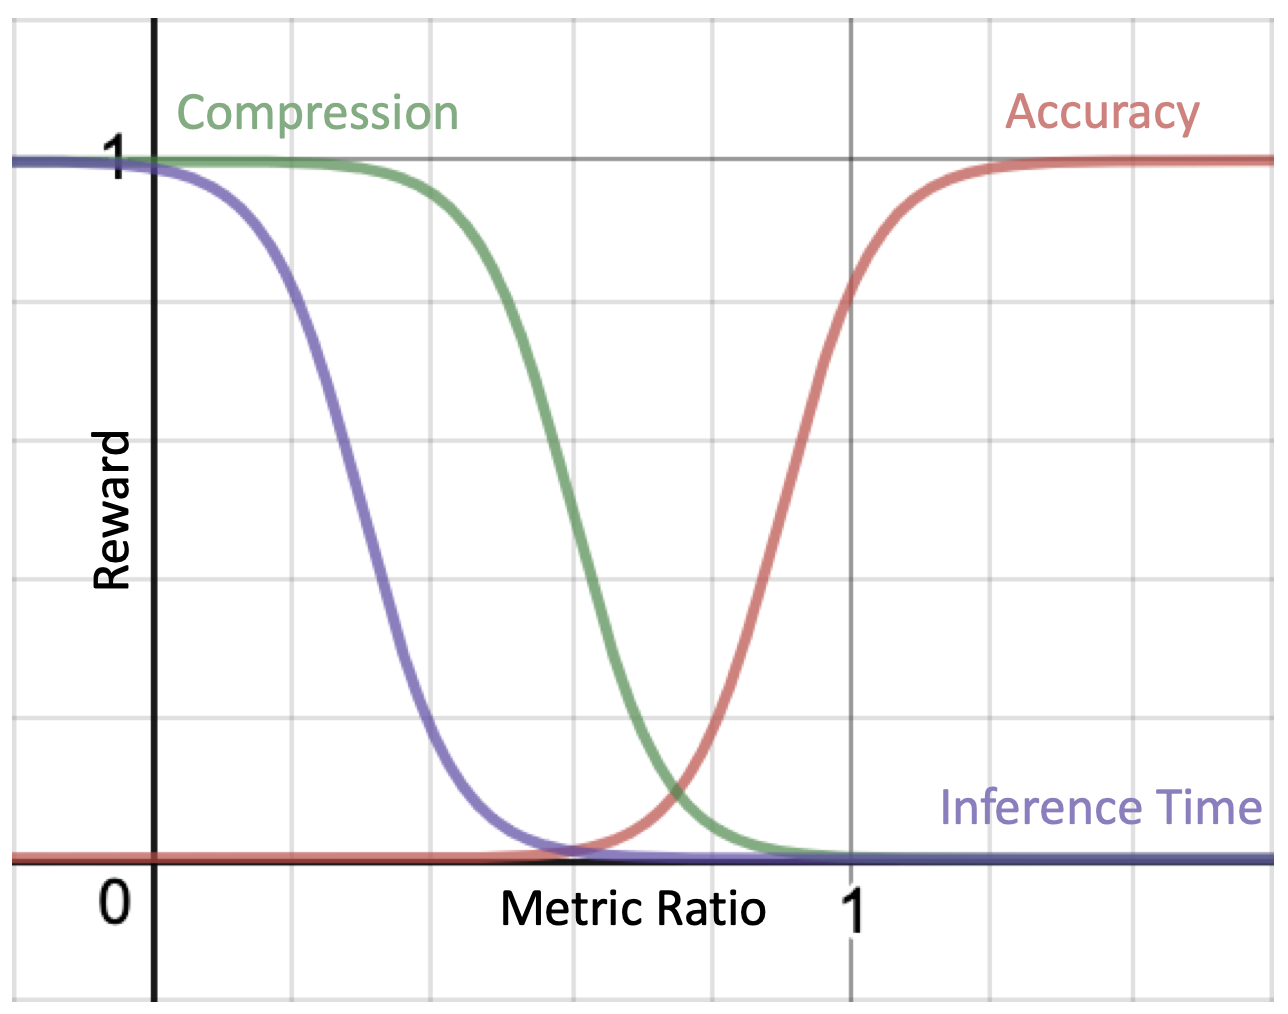
\includegraphics[width=0.95\figwidth]{rewardplot}
			\caption{Plot showing the reward structure of the 3 performance metrics}
			\label{fig:rewardfunction}
		\end{figure}
        An intelligently designed reward function which can differentiate between good and bad architectures is necessary for effective exploration in the architectural space.
        We introduce threshold-ed reward function which incorporates user specific device restriction, this allows us to reinforce the policy network to learn architectures which fit the device restrictions.
        Our objective is obtaining architectures which have high accuracy, low memory footprint as well as faster and computationally inexpensive at test time.
        Models having lower inference time (test time) and reasonably high accuracy are preferred over models with very high accuracy (in particular very deep models) which have higher inference time.
        Unlike previous work which optimize for indirect metrics such as FLOPS \cite{he2018amc}, we consider the inference latency on a single GPU as the measure of inference latency.
        We formulate a reward which is a combination three metrics for a given model $m$: Accuracy $A \bb{m}$, Compression percentage $C \bb{m}$ and Inference time $T \bb{m}$ (latency of model $m$) .
        We incorporate user specific device restrictions by introducing thresholds on Accuracy $A \bb{m}$ and Latency $T \bb{m}$.
        Incorporating real time latency in our reward allows us to effective search through the architectural space, resulting in model have high compression and reasonably high accuracy with the added benefit of lower inference time (which is essential element to be considered while deployment of the models to mobile devices)
        We perform intuitive transformation on accuracy Accuracy $A \bb{m}$, Compression percentage $C(m)$ and latency $T\bb{m}$ which are discussed in detail below.\\
        \textbf{Accuracy $A\bb{m}$:} Our primary objective is to obtain architectures which give high performance.
        One way to achieve this is by increasing the depth of the network \cite{he2015deep,simonyan2014very} but this comes at the expense of latency.
        We transform the reward obtained from accuracy such that we obtain a higher reward for model having high accuracy and is continuous function which provides flexibility to incorporate thresholds $A_{th}$ in the reward.
        Formally, reward is obtained through the following transformation.
        $R_1\fcolon A \rightarrow [0,1]$, which normalizes as well as enforces threshold to prevent exploration in undesired region of the search space.
            % \begin{equation}
            %     R_1 \bb{A} =    \begin{cases}
            %                     \log \frac{1}{2}\bb{1 + \exp\bb{\frac{A-A_{th}}{A_{teacher}}}}  &   a_{th} \leq a \leq 1    \\
            %                     \frac{A}{2*A_{teacher}}                               &   0 \leq a \leq a_{th}
            %                 \end{cases}
            % \end{equation} \\
            \begin{equation}
                R_1 \bb{A} = 1 - \inv{\bb{1+\exp\bb{15\cdot\bb{\frac{A}{A_{teacher}}-A_{th}}}}}
            \end{equation}
        where $A_{teacher}$ is accuracy of the teacher model. \\
        \textbf{Latency $T \bb{m}$ :} Inference Latency is essential component to considered which searching for a architecture fit for deployment.
        We incorporate the threshold by using a \textit{shifted sigmoid} transformation which is defined as : \\
        $R_2\fcolon T \rightarrow [0,1]$:
        % \begin{equation}
        %     R_2 \bb{T} =  \inv{\bb{1 + \exp\bb{10 \cdot (T-T_{th})}}}
        % \end{equation}
        \begin{equation}
                R_2 \bb{T} = \inv{\bb{1+\exp\bb{15\cdot\bb{\frac{T}{T_{teacher}}-T_{th}}}}}
        \end{equation}
        \textbf{Compression $C \bb{m}$ :} We use the ratio of the number of parameters of student and the teacher model and define the compression index as :\\
        $ C \bb{m} =  \#parameter(student)$, then similarly transform it to enforce our thresholds on size.\\
        % \begin{equation}
        %     R_3 \bb{C} = C \cdot (2 -C)
        % \end{equation}
         \begin{equation}
                R_3 \bb{C} = \inv{\bb{1+\exp\bb{15\cdot\bb{\frac{C}{C_{teacher}}-C_{th}}}}}
        \end{equation}
        Thresholds are needed as we search for the right balance in AMS trade-off Space the thresholds are $A_{th} = 0.9 $ $T_{th} = 0.3 $ $C_{th} = 0.6 $ are fixed for all of our experiments.
        As \textit{models with high degree of high compression does not guarantee lower inferences time}. The reward for the three performance metrics is given in~\ref{fig:rewardfunction}
        The final reward which need to be maximized for the RL process is defined as:
        \begin{equation}
        R \bb{m} = R_1 \bb{A\bb{m}}\cdot R_2 \bb{T\bb{m}} \cdot R_3 \bb{C\bb{m}}
        \end{equation}

        
    \subsection{Optimization}
        The parameters of the policy network characterized by $\theta$ are optimized to obtain a efficient policy to compress the teacher model.
        The optimization is formulated to maximize the \textit{expected reward} obtained from the newly compressed architecture defined as :
        \begin{equation}
            \theta^{*} = \arg \max_{\theta} E_{\bb{\Vec{s}, \Vec{a}} \sim p_{\theta\bb{\Vec{s}, \Vec{a}}}} \bb{R\bb{\Vec{s}}}
        \end{equation}
        \begin{equation} 
            J \bb{\theta} = E_{\bb{\Vec{s}, \Vec{a}} \sim p_{\theta\bb{\Vec{s}, \Vec{a}}}} \bb{R\bb{\Vec{s}}}
        \end{equation}
        where $R\bb{\Vec{s}}$ is total reward obtained.
        The optimization process can be estimated using REINFORCE policy gradient used in \cite{williams1992simple}, the continuous nature of our proposed reward transformation improves our search efficiency as it prevents exploding gradient.
        The gradient is estimated as:
        \begin{equation}
            \nabla_{\theta}  J \bb{\theta} = \nabla_{\theta} E_{\bb{\Vec{s}, \Vec{a}} \sim p_{\theta\bb{\Vec{s}, \Vec{a}}}} \bb{R\bb{\Vec{s}}}
        \end{equation}
        \begin{equation}
             \nabla_{\theta}  J \bb{\theta} \approx \frac{1}{N} \sum_{i = 1}^{N} \sum_{t = 1}^{T} \nabla_{\theta} \log{p_{\theta}\bb{a_{i,t}, s_{i,t}}} \bb{R\bb{\Vec{s}}}
        \end{equation}
        here $N$ represents number of produced architectures, $T$ represents the length of trajectory.
        The above equation has high variance, to normalize that we  utilize exponential moving average of the previous rewards as the baseline $b$ subtract it from our total reward $R\bb{\Vec{s}}$.
        \begin{equation}
             \nabla_{\theta}  J \bb{\theta} \approx \frac{1}{N} \sum_{i = 1}^{N} \sum_{t = 1}^{T} \nabla_{\theta} \log{p_{\theta}\bb{a_{i,t}, s_{i,t}}} \bb{R\bb{\Vec{s}} - b}
        \end{equation}
        This helps improve stability of the estimated gradients.

    \subsection{Knowledge Distillation}
    \label{sec:KD}
        Student model architectures are trained utilizing both the outputs of the teacher models and the true label.
        Instead of just using the un-normalized log probabilities (logits) of the teacher model, which outperforms the training process used in \cite{ashok2017n2n}.
        Training incorporating dark knowledge \cite{hinton2015distilling} that helps student to mimic the relationships learned by the teacher model.
        The loss function is trained as combination of \textit{hard} and \textit{soft} targets, giving higher  priority to transferring the dark knowledge.
        If $y_{i}$ are output logits of the teacher model of the $i^{th}$ training example, $y_{true}$ is the true labels.
        Then the loss function is described below as:
        \begin{align}
            \mathcal{L} & = \lambda\cdot\mathcal{L}_{soft} + \bb{1-\lambda}\cdot\mathcal{L}_{hard}   \\
            \mathcal{L}_{soft} & = D_{KL}\bb{f(x; W) \,\Vert\, y_{true}}    \notag \\
            & = \sum_{i} f(x^{i}; W) \cdot \log\frac{f(x^{i}; W)}{y_{true}(i)}   \\
            \mathcal{L}_{hard} & = H\bb{f(x; W), y} = - \sum_{i} f(x^{i}; W) \cdot \log{y_{i}}
        \end{align}
        
        Through experimentation we have fixed value of $\lambda = 0.7$ thus making the student model to mimic the behaviour of the teacher model simultaneously fine-tuning the student architecture towards the true labels.

    \subsection{Transferring Learned Compression Policy}
    \label{sec:TL}
        Unlike in the previous literature \cite{zoph2017learning, zoph2016neural} of transferring knowledge between different architecture families, we show transferability of the learned parameters of the policy across different subsets of data from a policy learned on the entire dataset .
        This not only provides a \textit{warm start} to the policy network but also improves upon the time to converge to good model architectures for given dataset (up to 5x reduction in time).
        Hence allowing us to get high performing compressed model architectures which satisfy user specific device thresholds, owing to the efficacy of transferring learnt information across dataset.
        Furthermore, we can train a policy for a larger dataset and subsequently fine tune the policy in a small data environment (often the case with data on mobile devices) to produce good architectures for the user tailored to the data.

\bibsubfile{named}{bibs/sub}
\end{document}

